%Emma Callery's Senior Seminar Paper

\documentclass{sig-alternate}
\usepackage{color}
\usepackage{listings}
\usepackage{url}
\usepackage{natbib}

\begin{document}
\conferenceinfo{UMM CSci Senior Seminar Conference, December 2014}{Morris, MN}
\title{Static and Dynamic Types in Software Development}
\numberofauthors{1}
\author{
\alignauthor
Emma G. Callery\\
	\affaddr{Division of Science and Mathematics}\\
	\affaddr{University of Minnesota, Morris}\\
	\affaddr{Morris, Minnesota, USA 56267}\\
	\email{calle052@morris.umn.edu}
}

\maketitle

\begin{abstract}
The debate between statically and dynamically typed languages has been going on since dynamic types were first introduced. Arguments have gone back and forth for everything from the benefits of both to what makes programmers hate one type system or the other. Unfortunately most arguments made for and against both type systems tend to come from personal opinion or personal experience. 
This paper takes a look at several studies that tried to look at this debate empirically to determine if either type system has an actual benefit to programmers. The first study looked at how programmers prefer to incorporate types in their programs when they have the chose. Several studies compared the time required to write out similar code in both a static and a dynamic language. 
The results are quite surprising, there are times where a static type system are faster. While there are other times dynamic typed systems are faster and even times where there is no determinable winner. All of this ultimately suggests that there is no superior type system, it is mostly determined by the programmer.  
\end{abstract}

\keywords{Static Types, Dynamic Types, Programming Languages, Java, Groovy.}

\section{Introduction}
Type systems (see \citep{Pierce2002}) have played an important role in programming languages since the beginning. Type systems effect everything from how new programmer are educated to what languages are used in industry and how. And while a great number of industry programming languages are statically typed (e.g.,Java), a fair number of programs use a dynamic type system (e.g.,Groovy). The later is especially common is web developments. This leads to the question of "whether one system or another, either static or dynamic, has a larger benefit for the humans that use them"\cite{Mayer2012}. This question has lead to a large debate of the benefits and draw-backs to both type systems, with people arguing strongly for both sides. The fault in many of these arguments is that most are not backed by empirical evidence but rather personal experience and opinions. Several studies have been conducted to try to determine if any of the arguments given(see section \ref{arguments}) have any real support.

This paper starts by defining what static and dynamic typed languages are in section \ref{types}, including arguments for both. Section \ref{programmers} looks at a study that tried to determine how programmers use types. Results of two studies that try to empirically determine the benefits of static types over dynamic types are covered in section \ref{benifits}. As the results of the last two studies were not as expected the overall results and the conclusions that can be drawn need to be discussed (section \ref{results}).

\section{Background Information}\label{types}
The key thing to know for this debate is the difference between static types and dynamic types. 

\subsection{Static Types}\label{static}
"A language is statically typed if the type of a variable is known at compile-time"\cite{NomeN2009}. For the type to be known at compile-time means that the programmer has \emph{declared} the type of the variable. Static languages compilers enforce these types by only allowing values of the declared type to be assigned to the variable. see Figure 1. This means that when the compiler goes through the code it not only checks other errors, but also checks for type errors.
 
\begin{figure}
\centering
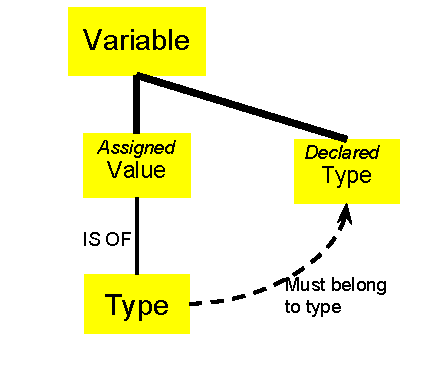
\psfig{file=Static_Type_Diagram.pdf,width =2in}
\caption{Diagram From Python Conquers the Universe of Static Types and Type Checking}
\end{figure}
\subsubsection{Arguments For Static Types}\label{arguments}
\begin{itemize}
\item Most error checking is done at compillookede-time, therefore catching errors more quickly.
\item Types help to communicate to the programmer and the programmer reason about the program.
\item Requiring type names act as a form of documentation or improves the quality of the documentation.
\item Improve the programs structure.
\end{itemize}



\subsection{Dynamic Types} \label{dynamic}
"A language is dynamically typed if the typlookede of a variable is interpreted at run-time"\cite{NomeN2009}. This is because types in dynamic languages are only associated with values\cite{Pierce2002}.see Figure 2. This does not mean that a type can not be associated with a variable, only that the language would not require the type be declared. This \emph{option} leads to what is called \emph{optional typing} where the programmer is primarily  responsible for the types incorporated in the program, as explained in section \ref{programmers}. 

\begin{figure}
\centering
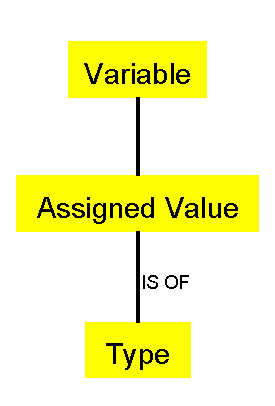
\psfig{file=Dynamic_Type_Diagram.pdf,width =1in}
\caption{Diagram From Python Conquers the Universe of Dynamic Types}
\end{figure}

\subsubsection{Arguments For Dynamic Types}
\begin{itemize}
\item More flexible, variables can be passed between functions more easily.
\item Without the need to declare every variable will make the program shorter, and therefore faster to write and read.
\item Programs without specific type requirements can be easily reused, with out having to write a whole new function to do the same thing to a different type
\item Not needing to declare variables, along with other 'administrative' commands, just to keep the compiler running allows for focusing to the conceptual concepts of the program.
\end{itemize}

\section{Programmer Preferences} \label{programmers}
This section will look at a study which attempted to determine where programmers use types and what types they used. The language used is the optional type language \emph{Groovy}. Groovy is a dynamically typed language that can access the static types in Java, claiming to "seamlessly integrate with existing Java classes" \cite{Souza2014}
\subsection{Study on Optional Typing}
Carlos Souza and Eduardo Figueiredo tried to understand programmer preferences in their paper \emph{How do Programmers Use Optional Typing? An Empirical Study}. In this study Souza and Figueiredo looked at 6638 projects written in the language Groovy. Looking over all of the projects Souza and Figueiredo tried to answer several questions about the use of types in the different projects.

\subsection{results of study on optional typing}


\section{Static V Dynamic Type Systems}\label{benifits}
\cite{Stuchlik2011}

\section{Influence}
\cite{Mayer2012}

\section{Conclusions}\label{results}
There are places where Dynamic is better then Static, and the surprising point where types no longer matter as much.

\section{Acknowledgments}


\bibliographystyle{abbrv}
\bibliography{My_paper.bib}


\end{document}
